\documentclass[border=10pt]{standalone}
\usepackage{pgfplots}
\pgfplotsset{compat=1.18}
\begin{document}
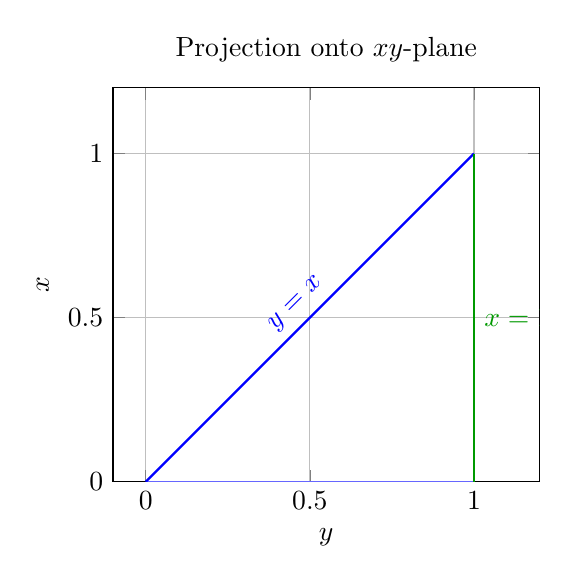
\begin{tikzpicture}
\begin{axis}[
    xlabel={$y$}, ylabel={$x$},
    xmin=-0.1, xmax=1.2, ymin=0, ymax=1.2,
    xtick={0,0.5,1}, ytick={0,0.5,1},
    title={Projection onto $xy$-plane},
    grid=both, width=7cm, height=7cm, axis equal image,
]
% Fill the triangular region: y in [0,1], x in [y,1]
\addplot[blue!30, draw=blue!60] coordinates {(0,0) (1,0) (1,1)} \closedcycle;
\addplot[blue, thick] coordinates {(0,0) (1,1)} node[above, sloped, midway] {$y=x$};
\draw[green!60!black, thick] (axis cs:1,0) -- (axis cs:1,1) node[right, midway] {$x=1$};
\end{axis}
\end{tikzpicture}
\quad
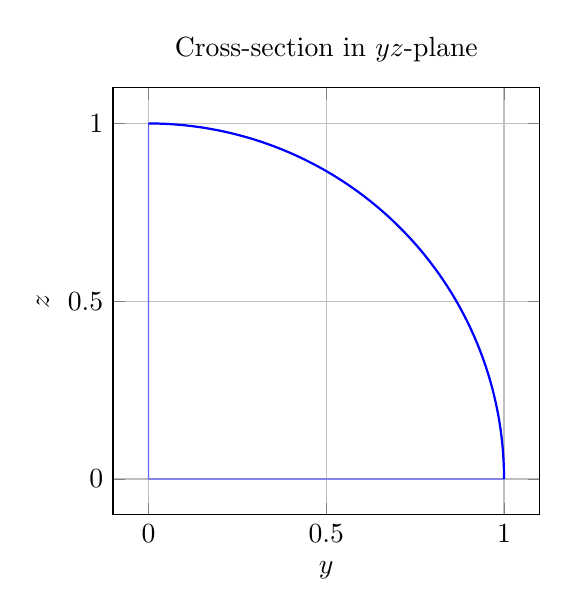
\begin{tikzpicture}
\begin{axis}[
    xlabel={$y$}, ylabel={$z$},
    xmin=-0.1, xmax=1.1, ymin=-0.1, ymax=1.1,
    xtick={0,0.5,1}, ytick={0,0.5,1},
    title={Cross-section in $yz$-plane},
    grid=both, width=7cm, height=7cm, axis equal image,
]
% Quarter disk in yz-plane (since cylinder is y^2+z^2=1, z>=0, y>=0)
\addplot[blue!30, draw=blue!60, domain=0:90, samples=80] ({cos(x)}, {sin(x)}) \closedcycle;
\addplot[blue, thick, domain=0:90, samples=80] ({cos(x)}, {sin(x)});
\end{axis}
\end{tikzpicture}
\end{document}